% Prototype status and preliminary results (issue #13).

\section{Prototype Status}
Every Phase~1 module is complete and integrated: the MAC unit, the PE, the $N \times N$ array, the input skew buffers, the output buffer, the controller and the top level. All seven RTL files pass Verilator lint with every warning enabled, and every module has a self-checking testbench. Table~\ref{tab:tests} lists the checks each testbench makes in the current regression, \texttt{make lint test} on \texttt{dev}: 10{,}349 checks, none failed. The same command runs in continuous integration on every pull request. The logs of the buffer, array and end-to-end tests are kept in \path{results/phase1/logs/}.

\begin{table}[t]
\centering
\caption{Testbench results, \texttt{make lint test} on \texttt{dev}}
\label{tab:tests}
\footnotesize
\begin{tabular}{@{}llr@{}}
\toprule
Testbench & Module under test & Checks passed \\
\midrule
\texttt{tb\_mac} & MAC unit & 20/20 \\
\texttt{tb\_pe} & processing element & 15/15 \\
\texttt{tb\_sa\_controller} & controller & 56/56 \\
\texttt{tb\_input\_skew\_buffer} & input skew buffer & 496/496 \\
\texttt{tb\_output\_buffer} & output buffer & 96/96 \\
\texttt{tb\_systolic\_array} & $4 \times 4$ and $3 \times 3$ array & 7{,}471/7{,}471 \\
\texttt{tb\_systolic\_top} & complete accelerator & 2{,}195/2{,}195 \\
\midrule
Total & & 10{,}349/10{,}349 \\
\bottomrule
\end{tabular}
\end{table}

The end-to-end test drives the accelerator only through its host ports. It loads each of the 106 golden cases, runs it, and compares every element of $C$ with the golden model; every element of every case matches. It also checks the handshake rules: writes during a run are ignored, back-to-back runs work, one matrix can be replaced on its own, $C$ stays readable until the next capture, and a reset during a run returns the accelerator to idle.

\subsection{Measured Latency}
For every case the testbench counts the cycles in which \texttt{busy} is high and reads \texttt{cycle\_count} when \texttt{done} rises. Both are 12 in all 106 runs, recorded in \path{results/phase1/cycle_counts.csv}: one \texttt{CLEAR} cycle, $T = 10$ compute cycles and one \texttt{CAPTURE} cycle, exactly as the timing contract predicts. Fig.~\ref{fig:array-wave} shows the computation inside the array on the known product: the operands enter along the skewed edges and the results fill in diagonal by diagonal, with PE $(3,3)$ finishing in the last compute step.

\begin{figure*}[t]
\centering
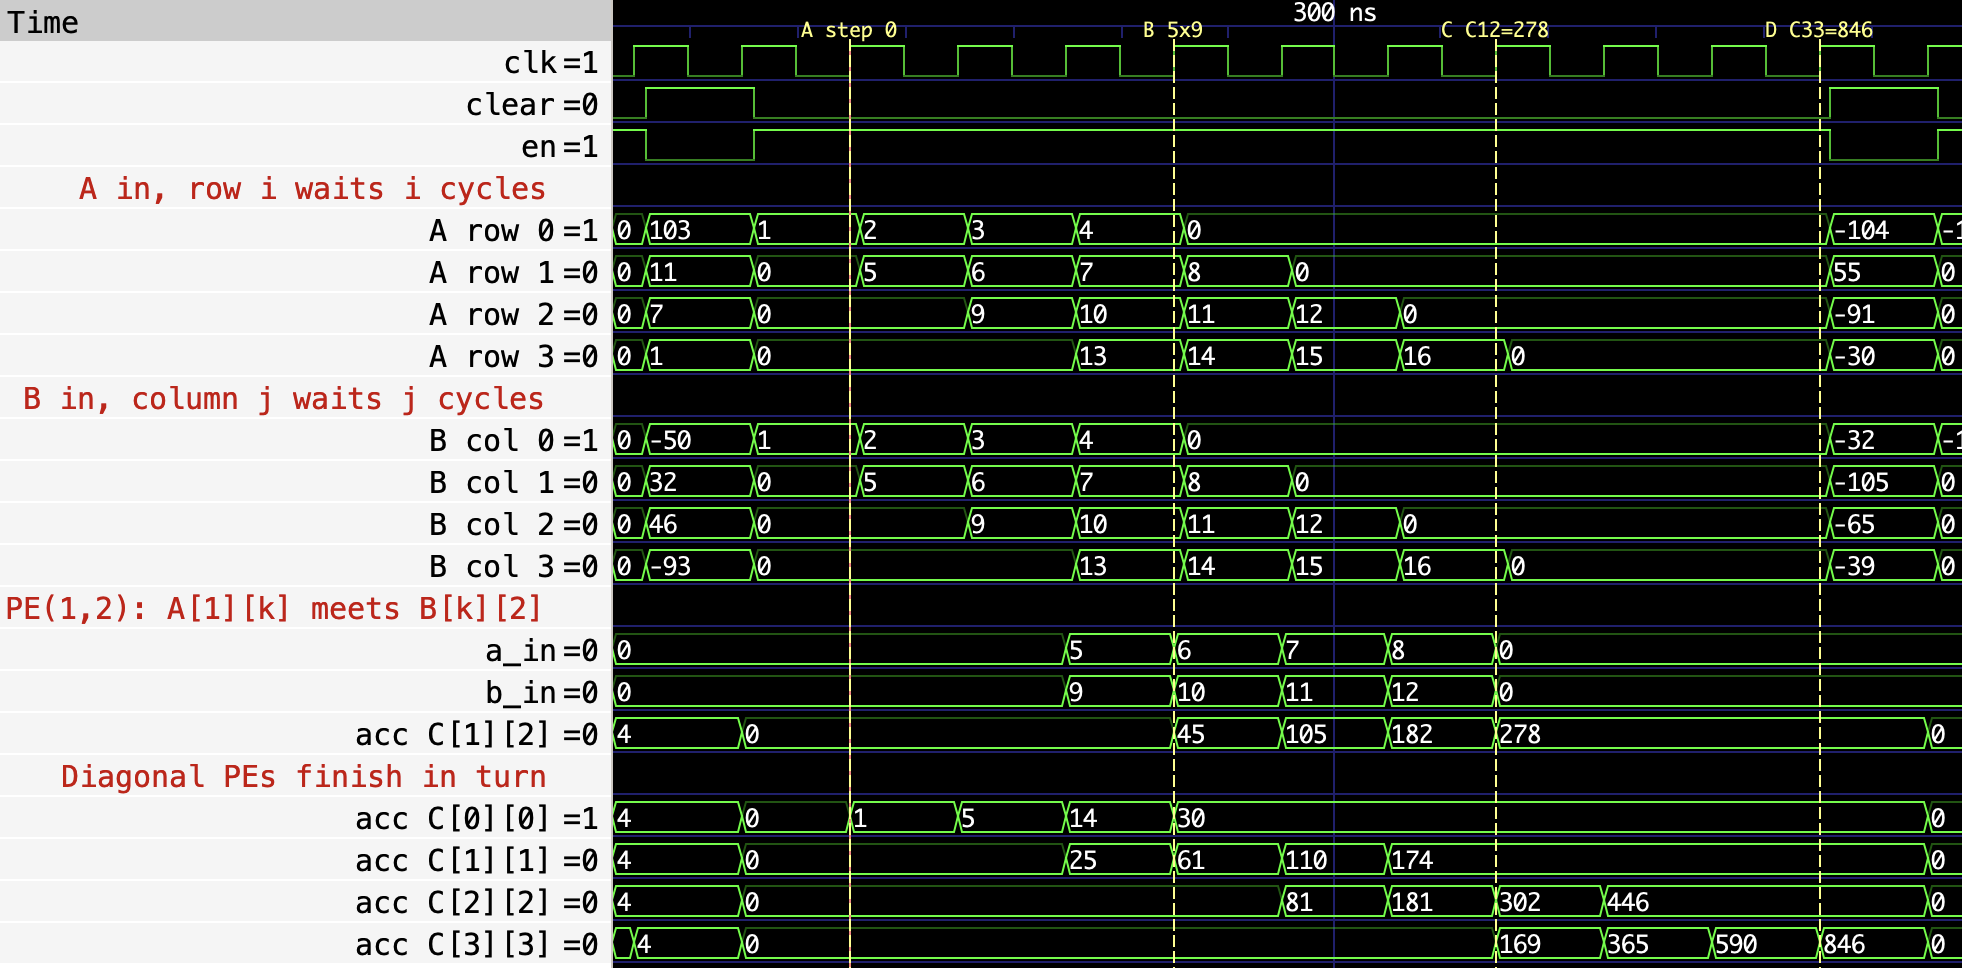
\includegraphics[width=0.82\textwidth]{systolic_array.png}
\caption{The $4 \times 4$ array on the known product ($A = 1, \ldots, 16$ in row-major order, $B = A^{\mathsf T}$), from \texttt{tb\_systolic\_array}. Row $i$ of $A$ and column $j$ of $B$ enter $i$ and $j$ cycles late, so $A[1][k]$ meets $B[k][2]$ at PE $(1,2)$ from marker B on and gives $C[1][2] = 278$ (C). PE $(3,3)$ finishes $C[3][3] = 846$ in the last step, $T - 1 = 9$ (D). Values during \texttt{CLEAR} are random and ignored.}
\label{fig:array-wave}
\end{figure*}

\subsection{Comparison with a Sequential MAC}
A single sequential MAC unit needs one cycle per multiply-accumulate, so an $N \times N$ product with $K = N$ takes $N^3 = 64$ cycles. Table~\ref{tab:perf} compares it with the measured array. The array performs the same 64 MACs in 10 compute cycles, 6.4 on average per cycle against a peak of 16, so it needs 6.4 times fewer compute cycles, and 5.3 times fewer counting all 12 busy cycles. The gap grows with the array: the sequential unit needs $N^3$ cycles and the array $3N - 2$, so for $N = 8$ the compute ratio would be $512/22 \approx 23$. These baseline figures are analytical; a sequential RTL baseline, synthesis and clock-frequency results are Phase~2 work. Loading the operands and reading the result through the one-element ports adds 32 cycles per product, so at this size the ports, not the array, limit end-to-end throughput.

\begin{table}[t]
\centering
\caption{Measured array latency against one sequential MAC ($N = K = 4$)}
\label{tab:perf}
\footnotesize
\begin{tabular}{@{}lrr@{}}
\toprule
Metric & Sequential MAC & Systolic array \\
\midrule
MACs per product & 64 & 64 \\
Compute cycles & 64 & 10 \\
Cycles from \texttt{start} to \texttt{done} & -- & 12 \\
MACs per compute cycle, average & 1 & 6.4 \\
MACs per cycle, peak & 1 & 16 \\
Speed-up, compute cycles & 1 & 6.4 \\
Speed-up, \texttt{start} to \texttt{done} & 1 & 5.3 \\
\bottomrule
\end{tabular}
\end{table}
